\chapter{Metodologia}
% ---
Neste capítulo serão apresentados as linguagens de programação, equipamentos e \textit{softwares} utilizados na construção do sistema proposto.
% ---
\section{Linguagens de programação}

As linguagens de programação que foram utilizadas para a implementação do sistema estão presentes nesta seção.
\subsection{Python}

Python é uma linguagem de programação interpretada, de alto nível e de uso geral. Criado por Guido van Rossum e lançado pela primeira vez em 1991, a filosofia de design do Python enfatiza a legibilidade do código com seu uso notável de espaço em branco significativo. Suas construções de linguagem e abordagem orientada a objetos têm como objetivo ajudar os programadores a escrever código claro e lógico para projetos de pequena e grande escala.

O Python suporta vários paradigmas de programação, incluindo programação estruturada (principalmente processual), orientada a objetos e funcional. O Python é frequentemente descrito como uma linguagem "baterias incluídas" devido à sua abrangente biblioteca padrão.

Os intérpretes de Python estão disponíveis para muitos sistemas operacionais. Uma organização sem fins lucrativos, a Python Software Foundation, gerencia e direciona recursos para o desen
volvimento de Python. \cite{van2007python}

\subsection{Node.JS}


O Node.JS, também conhecido como Node, é uma estrutura EDA de código aberto para o desenvolvimento de aplicativos JavaScript em servidores. É baseado no \textit{runtime} do Google, chamado de motor V8. O V8 e o Node são implementados em C e C++, focados no desempenho e baixo consumo de memória. Embora o V8 suporte principalmente o uso de JavaScript no navegador, o Node foca no suporte de processos de servidores \cite{Tilkov2010}.

O EDA é uma maneira de realizarmos a comunicação entre sistemas que consiste, principalmente em operações assíncronas além de permitir aplicativos escalonáveis e gerar menos acoplamento entre os serviços, permitindo uma arquitetura fortemente flexível. 

O Node é um dos ambientes e \textit{frameworks} mais famosos que suportam o desenvolvimento de servidores utilizando o JavaScript \cite{Tilkov2010}.

\subsection{HTML}

De acordo com \citeauthor{html}, para publicar informações para distribuição global, é preciso uma linguagem universalmente compreendida, um tipo de publicação na língua materna que todos os computadores possam entender. A linguagem de publicação usada pela WWW\footnote{WWW é um sistema de documentos dispostos na Internet que permitem o acesso às informações apresentadas no formato de hipertexto.} é HTML (da HyperText Markup Language). 

O HTML fornece aos autores os meios para: 
\begin{itemize}
    \item Publicar documentos on-line com títulos, texto, tabelas, listas, fotos, etc. 
    \item Recuperar informações on-line por meio de links de hipertexto, com o clique de um botão. 
    \item Crie formulários para realizar transações com serviços remotos, para uso em busca de informações, reservas, pedidos de produtos, etc. 
    \item Inclua planilhas, videoclipes, clipes de som e outros aplicativos diretamente em seus documentos.
\end{itemize}

\subsection{CSS}
De acordo com \citeauthor{css}, um dos padrões fundamentais do W3C \footnote{O padrão W3C trata-se de uma organização internacional com mais de 400 membros, entre empresas, órgãos governamentais e associações independentes, responsável pelos protocolos e padronização da WWW, a rede mundial de computadores.} para o desenvolvimento de aplicativos da web é o \textit{Cascading Style Sheets}(CSS) \cite{Casca8378199:online}. CSS é uma linguagem para definir a semântica de apresentação dos elementos HTML, incluindo seu posicionamento, layout, cor e fontes. A principal força motriz por trás da adoção do CSS tem sido a separação da estrutura da apresentação. Embora essa separação de preocupações ajude a evolução de um aplicativo da Web no que diz respeito à estrutura e ao conteúdo, o código CSS em si não é fácil de manter \cite{badros1999constraint}. 

Escrever código CSS não é trivial \cite{quint2007editing}. Requer interação humano-computador, design gráfico, além de habilidades de programação na web \cite{keller2010css}. Além disso, a linguagem possui várias características, como especificidade de herança, cascata e seletor, o que torna o entendimento de como as propriedades CSS são aplicadas aos elementos DOM em tempo de execução, uma tarefa assustadora para desenvolvedores da web.


\section{Métodos}

Os métodos e conceitos que foram utilizados para a implementação do sistema estão presentes nesta seção.

\subsection{\textit{Bounding Box}}

As \textit{Bounding Box}(bbox) (Figura \ref{fig:boundingBox}) são um dos métodos de anotação de imagem mais populares e reconhecíveis usados em \textit{Machine Learning} e em \textit{Deep Learning}.

Elas são caixas retangulares que podem ser determinadas pelas coordenadas dos eixos x1 e y1 no canto superior esquerdo e as coordenadas dos eixos x2 e y2 no canto inferior direito do retângulo. Com exemplo, definiremos as \textit{Bounding Boxes} do cachorro e do gato com base nas informações de coordenadas da imagem real .\cite{allDeep}

\begin{figure}[htbp]
		\centering
		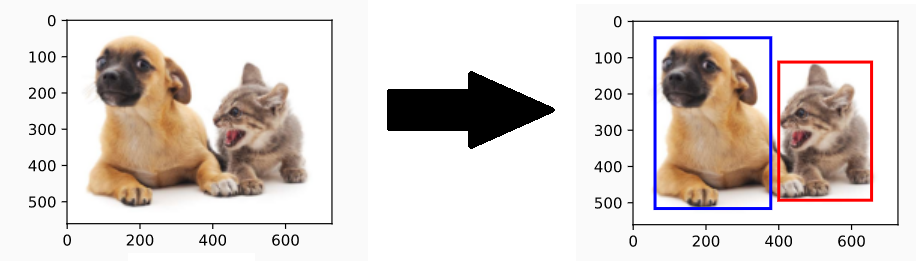
\includegraphics[scale=0.4]{figuras/MachineLearning/catDog.png}
		\caption{Execução de \textit{Bounding Boxes}.}
		\legend{Fonte: \cite{133Ob9905723:online})}
		\label{fig:boundingBox}
\end{figure}

O código \ref{cod:bbox} refere-se à posição das \textit{Bounding Boxes} do cachorro e do gato na imagem, respectivamente.

\begin{lstlisting}[caption=Posições de X e Y nas \textit{Bounding Boxes}, label=cod:bbox]
         dog_bbox, cat_bbox = [60, 45, 378, 516], [400, 112, 655, 493]
\end{lstlisting}


\subsection{\textit{Data Augmentation}}

\textit{Data Augmentation} é o processo de aumentar a quantidade e a diversidade de dados. A partir de imagens originais, gerar mais imagens semelhantes através de vários métodos como girar 25º, 90º, 45º, embaçar a imagem, entre outros para que possa agrupar em um dataset mais robusto.

Quanto mais dados um algoritmo de ML tiver acesso, mais eficaz ele poderá ser. Mesmo quando os dados são de qualidade inferior, os algoritmos podem ter um desempenho melhor, desde que dados úteis possam ser extraídos pelo modelo do conjunto de dados original. Por exemplo, os modelos de conversão de texto em fala e em texto melhoraram significativamente devido ao lançamento de um corpus de trilhões de palavras pelo Google \cite{halevy2009unreasonable}. Esse resultado ocorre apesar dos dados serem coletados de páginas da Web não filtradas e conter muitos erros. Com esses conjuntos de dados grandes e não estruturados, no entanto, a tarefa passa a ser a de encontrar estrutura dentro de um mar de dados não estruturados. \cite{dataAug}

\subsection{TensorFlow}

O TensorFlow é uma interface para expressar algoritmos de \textit{Machine Learning} e uma implementação para a execução de tais algoritmos. Um cálculo expresso usando o TensorFlow pode ser executado com pouca ou nenhuma alteração em uma ampla variedade de sistemas heterogêneos, desde dispositivos móveis como telefones e tablets até sistemas distribuídos em larga escala de centenas de máquinas e milhares de dispositivos computacionais, como Placas de GPU. 

O sistema é flexível e tem sido usado para conduzir pesquisas e implantar sistemas de aprendizado de máquina na produção em mais de uma dúzia de áreas da ciência da computação e outros campos, incluindo reconhecimento de fala, visão computacional, robótica, recuperação de informações, processamento de idiomas, extração de informações geográficas e descoberta computacional de drogas. \cite{abadi2016tensorflow}

Vários serviços do Google uilizam o TensorFlow em sua produção, o lançaram como um projeto de código aberto e
tornou-se amplamente utilizado para pesquisa de ML.\cite{199317}

\subsection{Scikit-Image}

O Scikit-image, também conhecido como Skimage, é uma biblioteca de processamento de imagens que implementa algoritmos e utilitários para uso em aplicações de pesquisa, educação e indústria. É lançado sob a licença liberal de código aberto Modified BSD, fornece uma API bem documentada na linguagem de programação Python e é desenvolvido por uma equipe internacional ativa de colaboradores.

O objetivo do scikit-image é fornecer uma biblioteca de alta qualidade de ferramentas poderosas e diversas de processamento de imagens, gratuitas e sem restrições. Esses princípios são a base para as práticas de desenvolvimento na comunidade de imagens scikit.\cite{skimage}

\subsection{ImageAI}

ImageAI é uma biblioteca python de código aberto criada para capacitar os desenvolvedores a criar aplicativos e sistemas com recursos independentes de \textit{Deep Learning} e \textit{Computer Vision} usando simples e poucas linhas de código.

A biblioteca ImageAI suporta previsão e treinamento de imagens usando 4 algoritmos diferentes de \textit{Machine Learning} treinados no conjunto de dados ImageNet-1000. O ImageAI também suporta detecção de objetos, detecção de vídeo e rastreamento de objetos usando RetinaNet, YOLOv3 e TinyYOLOv3 treinados no conjunto de dados COCO e PASCAL VOC.\cite{ImageAI}

Neste trabalho será utilizada uma classe da biblioteca ImageAI chamada \textit{Custom Detection Model Training}, possibilitando o treinamento do meu próprio modelo de detecção de objetos utilizando a arquitetura da YOLOv3.

\subsection{YOLOv3}

A rede neural YOLOv3 evoluiu de YOLO e YOLO-V2 \cite{redmon2018yolov3}. Quando comparado com a rede Faster R-CNN, a mais eficiente das CNNs quando, a YOLO transforma o problema de detecção em um problema de regressão, em que a informação tem um significado numérico resultante de alguma previsão na imagem. Isto não requer uma região da proposta e gera coordenadas e probabilidades de \textit{bounding boxes} (\textit{bbox}) de cada classe diretamente por meio de regressão. Isso aumenta consideravelmente a velocidade de detecção em comparação com o Faster R-CNN.\cite{yolov3_apple}

O YOLO é uma ordem de magnitude mais rápida (45 \textit{frames} por segundo) do que outros algoritmos de detecção de objetos \cite{yolov3RealTime}. Comparando a rede Faster R-CNN com a  R-CNN, a velocidade do treinamento  é 9 vezes mais rápida e a velocidade do teste é 213 vezes mais rápida. \cite{7960069}

O YOLO impõe fortes restrições espaciais nas previsões de \textit{bbox}, pois cada célula da \textit{grid} prevê apenas duas \textit{box} e pode ter apenas uma classe. Essa restrição espacial limita o número de objetos próximos que o modelo pode prever. O modelo luta com pequenos objetos que aparecem em grupos, como por exemplo, bandos de pássaros. \cite{yolov3RealTime}

\begin{figure}[htbp]
		\centering
		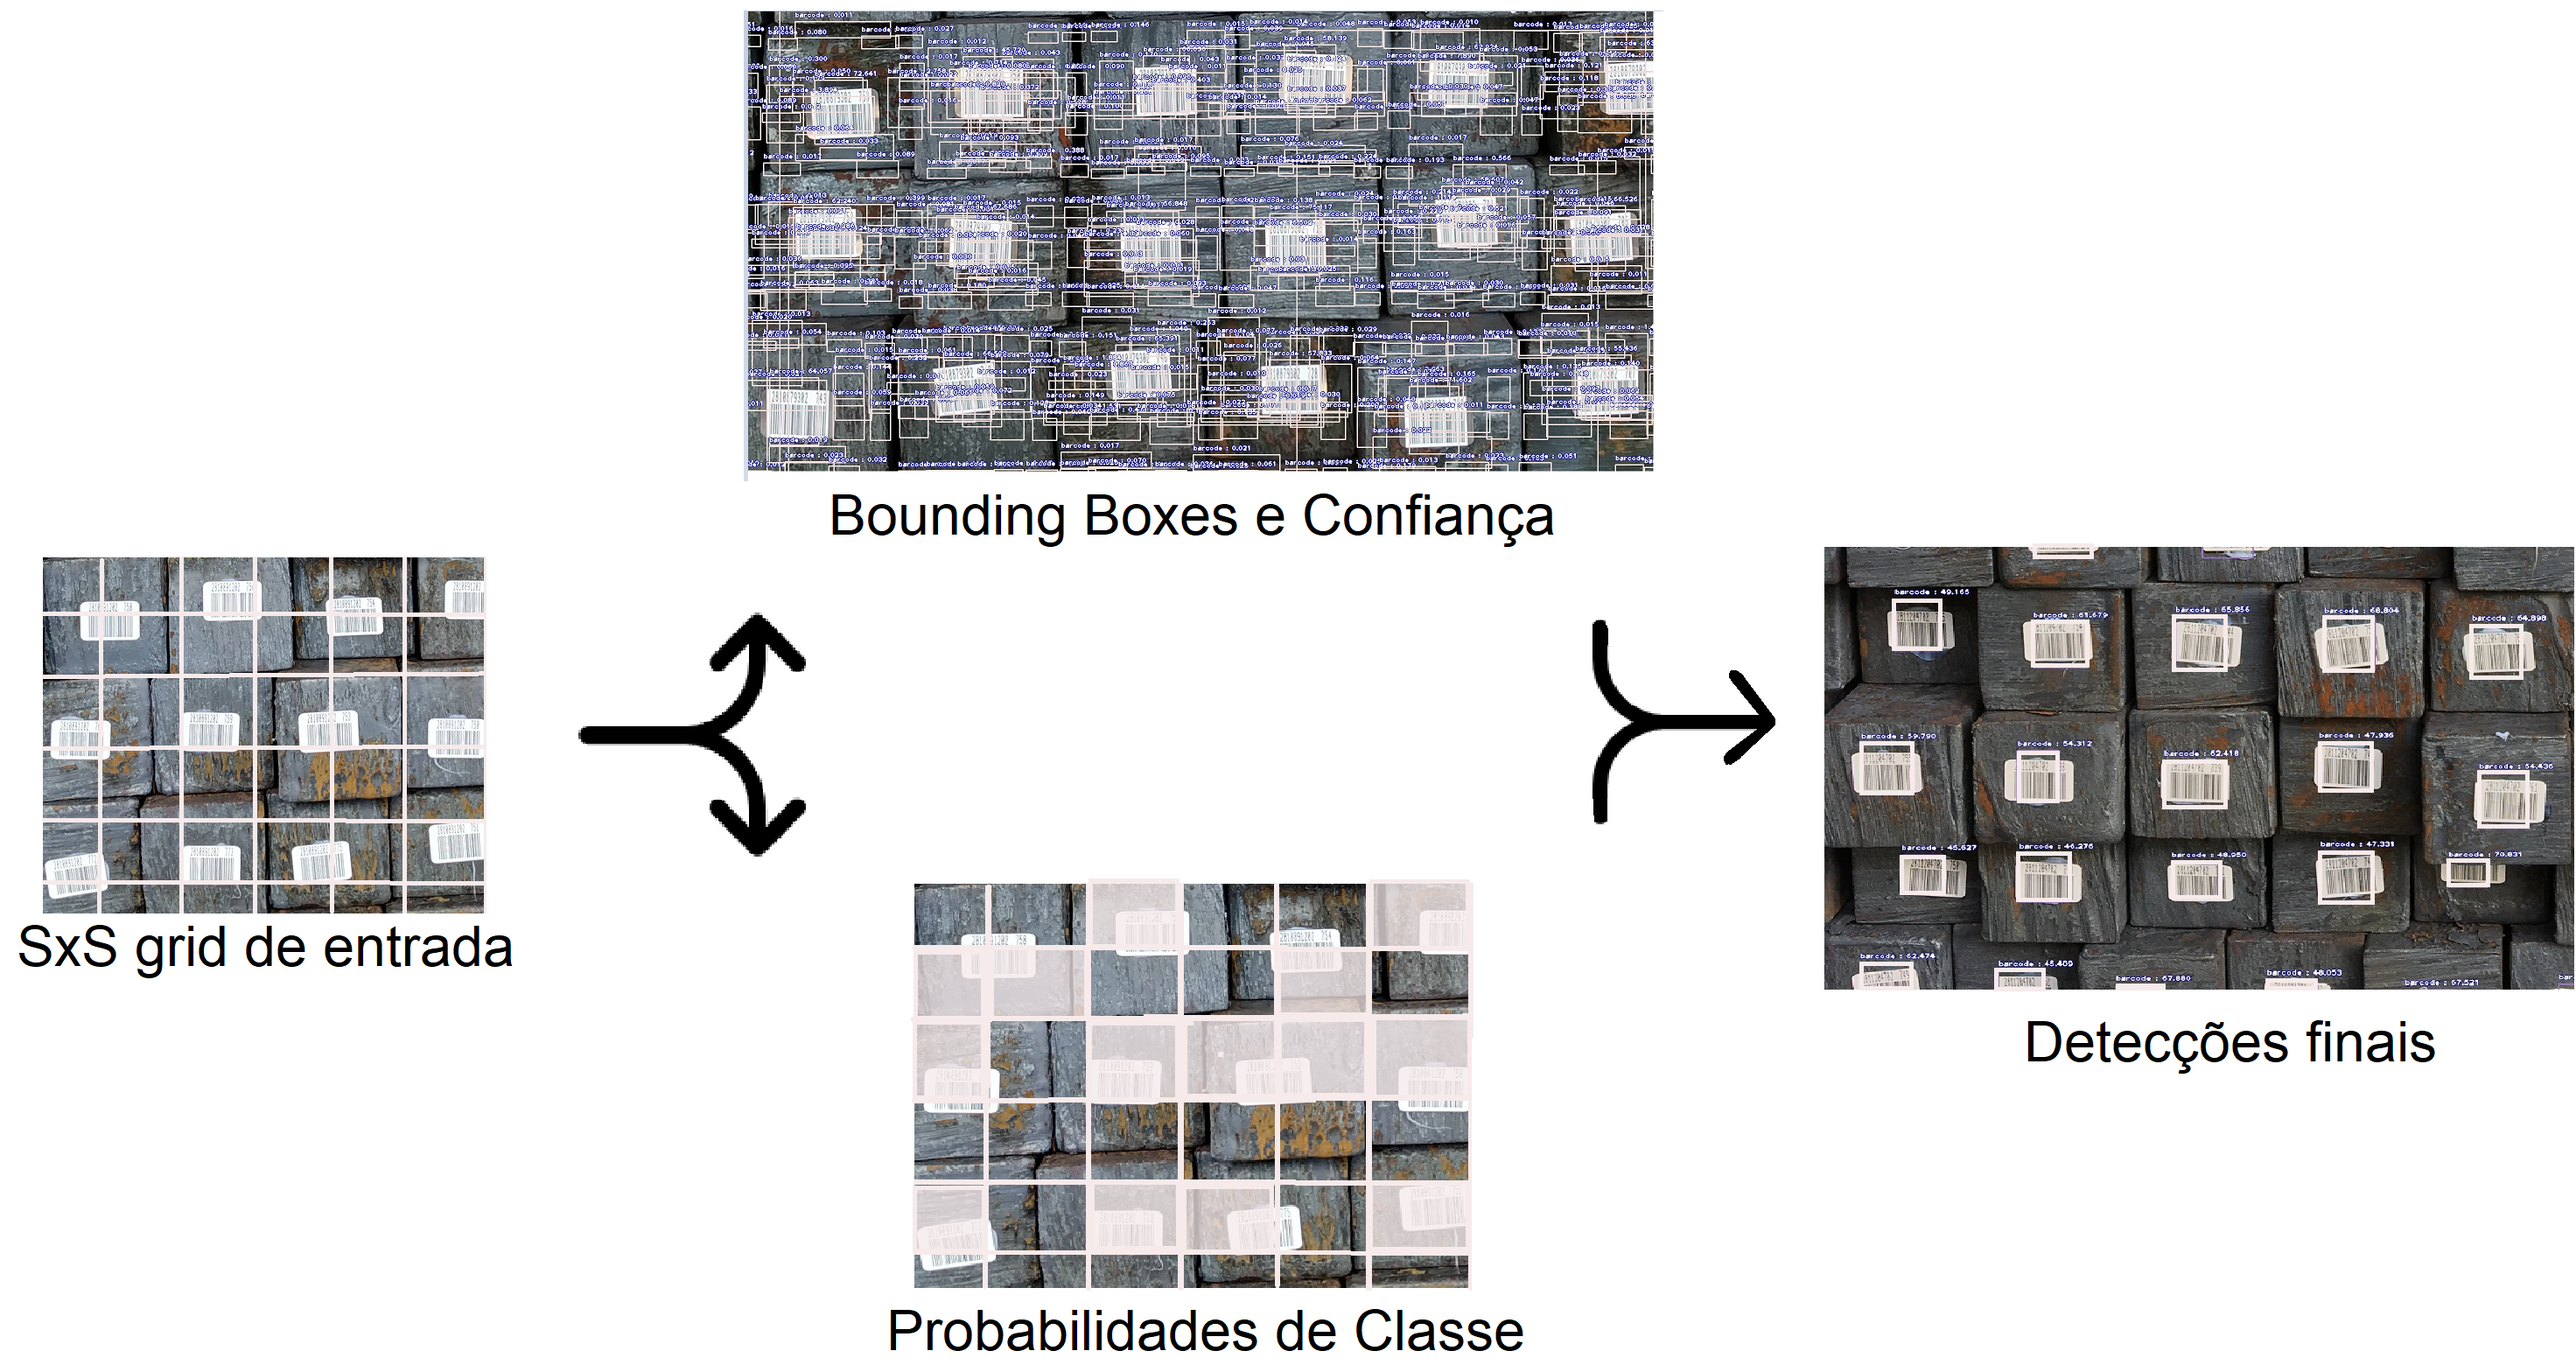
\includegraphics[scale=0.2]{figuras/MachineLearning/yolo.png}
		\caption{YOLO}
		\label{fig:yolo}
\end{figure}

No modelo de detecção YOLO (Figura \ref{fig:yolo}) uma única rede convolucional prediz tanto os \textit{bounding boxes} quanto as probabilidades de pertinencia a classe de cada objeto detectado. Para isso, YOLO funciona da seguinte forma:

\begin{itemize}
    \item Toma-se uma imagem e divide-se-a em um grid SxS de células (S = 6);
    \item Usando o \textit{grid} como referência, gera-se N \textit{bounding boxes};
    \item \textit{Bounding boxes} com probabilidade acima de um limiar são selecionados e usados para localizar o objeto dentro da imagem.
\end{itemize}

Cada célula do  \textit{grid} é usada para predizer B  \textit{bbox} e C probabilidades de classe. O conceito de interseção sobre união (IoU) tem um papel importante e a confiança de uma predição em YOLO é dada por:

%\begin{equation}
    
%\end{equation}

% TODO hey, jogue essa equação na estrutura que coloquei acima.
\[Confianca = p_r(Object) X IoU_{pred}^{truth} , p_r(Object) \in \left \{ 1\right.,\left.0\right \}\]

Em que, quando o \textit{target} estiver na \textit{grid}, \(p_r(Object)\) = 1 e 0 caso contrário. \(IoU_{pred}^{truth}\) é usado para denotar a interseção sobre união e a previsão da \textit{bbox}. A confiança reflete se a \textit{grid} contém objetos e a precisão da \textit{bbox} prevista. Quando várias \textit{bbox} detectam o mesmo \textit{target}, o YOLO usa o método de não supressão máxima (NMS) para selecionar a melhor \textit{bbox}.

\subsection{OpenCV}

O OpenCV (Open Source Computer Vision) é uma biblioteca de \textit{open source} e \textit{cross-plataform} (Multiplataforma) que contém mais de 500 algoritmos otimizados para análise de imagem e vídeo. Desde sua introdução em 1999, ele foi amplamente adotado como a principal ferramenta de desenvolvimento pela comunidade de pesquisadores e desenvolvedores em visão computacional. O OpenCV foi originalmente desenvolvido na Intel por uma equipe liderada por Gary Bradski como uma iniciativa para avançar na pesquisa em visão e promover o desenvolvimento de aplicativos intensivos em CPU e baseados em visão. Após lançamentos de varias versões Beta,  a Version 1.0 foi lançada em 2006. Um segundo grande lançamento ocorreu em 2009 com o lançamento do OpenCV 2, que propunha mudanças importantes, especialmente a nova interface C++. Em 2012, o OpenCV reformulou sua fundação que hoje depende do financiamento coletivo para seu desenvolvimento futuro. \cite{opencv}

\section{Softwares}
Os softwares que foram utilizados para a implementação do sistema estão presentes nesta seção.
% ---
\subsection{Google Colaboratory}
O Google Colaboratory, mais conhecido como "Google Colab" ou simplesmente "Colab", é um projeto de pesquisa para criar protótipos de modelos de \textit{Machine Learning} em poderosas opções de \textit{hardware}, como GPUs e TPUs. Ele fornece um ambiente de notebook Jupyter sem servidor para desenvolvimento interativo. O Google Colab é gratuito para usar como outros produtos do G Suite — que anteriormente era conhecido como Google Apps — no qual é um serviço oferecido pelo Google que fornece diversas ferramentas da própria empresa. Elas podem ser totalmente personalizadas com as informações do negócio, incluindo um domínio próprio.

Além de ser fácil de usar, o Colab é bastante flexível em sua configuração e faz muito do trabalho pesado para você. \cite{colabdetail}

\begin{itemize}
    \item Suporte para Python 2.7 e Python 3.6;
    \item Aceleração de GPU;
    \item Bibliotecas pré-instaladas: Todas as principais bibliotecas Python, como o TensorFlow, o Scikit-learn, o Matplotlib, entre muitas outras, estão pré-instaladas e prontas para serem importadas;
    \item Construído com base no Jupyter Notebook;
    \item Recurso de colaboração (funciona com uma equipe igual ao Google Docs): o Google Colab permite que os desenvolvedores usem e compartilhem o Jupyter notebook entre si sem precisar baixar, instalar ou executar qualquer coisa que não seja um navegador;
    \item Suporta comandos \textit{bash};
    \item Os notebooks do Google Colab são armazenados no drive.
\end{itemize}

\begin{figure}[htbp]
		\centering
		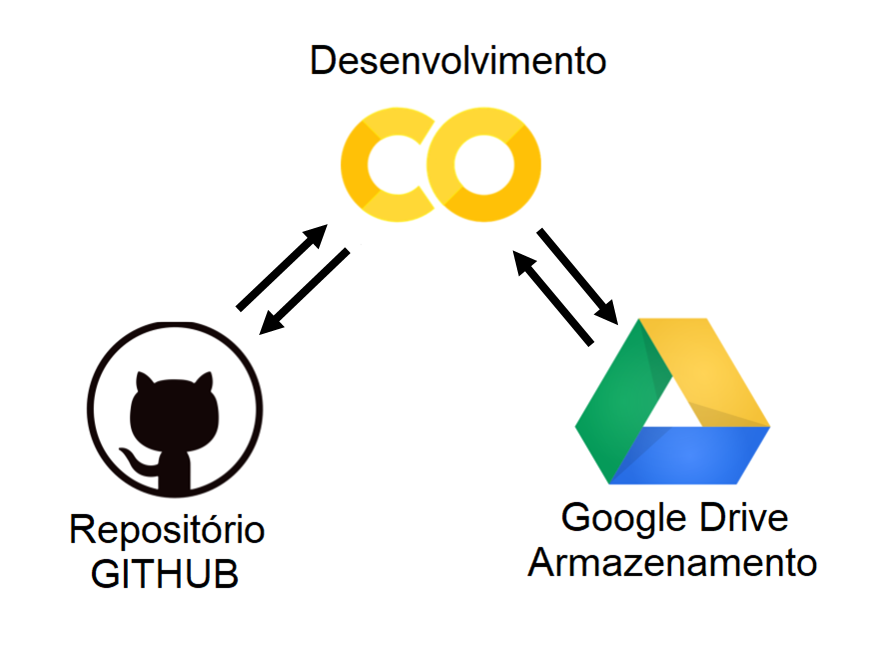
\includegraphics[scale=0.4]{figuras/MachineLearning/colabGithub.png}
		\caption{Utilização do Colab, Drive e Github}
		\label{fig:colabGithub}
\end{figure}

O Colab se integra facilmente ao Google Drive, o que o torna uma opção natural para espaço de armazenamento, em que se armazena os dados e os modelos. Ao mesmo tempo, o Github é mais adequado para hospedagem de código e uso de diversas  bibliotecas gratuitas disponíveis pela comunidade. 

\subsection{LabelImg}

O labelImg (Figura \ref{fig:labelimg}) é uma ferramenta open source de anotação de imagem gráfica escrita em Python. As anotações são salvas em arquivos XML no formato PASCAL VOC (Figura \ref{fig:labelXml}), o formato usado pelo ImageNet. Além disso, também suporta o formato YOLO no qual utilizaremos em nosso projeto. \cite{labelimg}

O software em questão permite que você circule as \textit{bounding boxes} englobando o objeto de interesse nas imagens e criando automaticamente um arquivo XML com todas as especificações necessárias.

Utiliza-se a ferramenta para formar o \textit{dataset}, que é um dos fundamentos da \textit{deep learning}. Para muitos pesquisadores obter dados suficientes para realizar o experimento por si só é um grande problema, por isso precisamos de muitos \textit{datasets open source} para que todo mundo possa usar. Alguns \textit{datasets} comumente usados na visão computacional são os seguintes.

\begin{figure}[htbp]
	\centering
	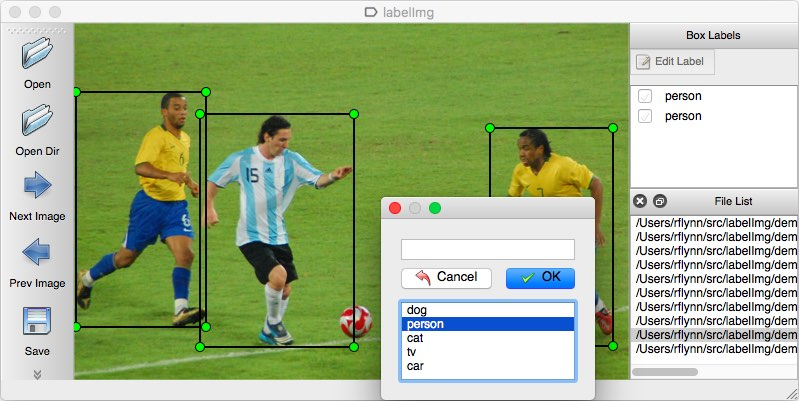
\includegraphics[width=0.9\linewidth]{figuras/MachineLearning/labelimg.jpg}
	\caption{Procedimento de anotações das \textit{bounding boxes}}
	\legend{Fonte: \citeauthor{labelimg} (\citeyear{labelimg})}
	\label{fig:labelimg}
\end{figure}

\begin{figure}[htbp]
	\centering
	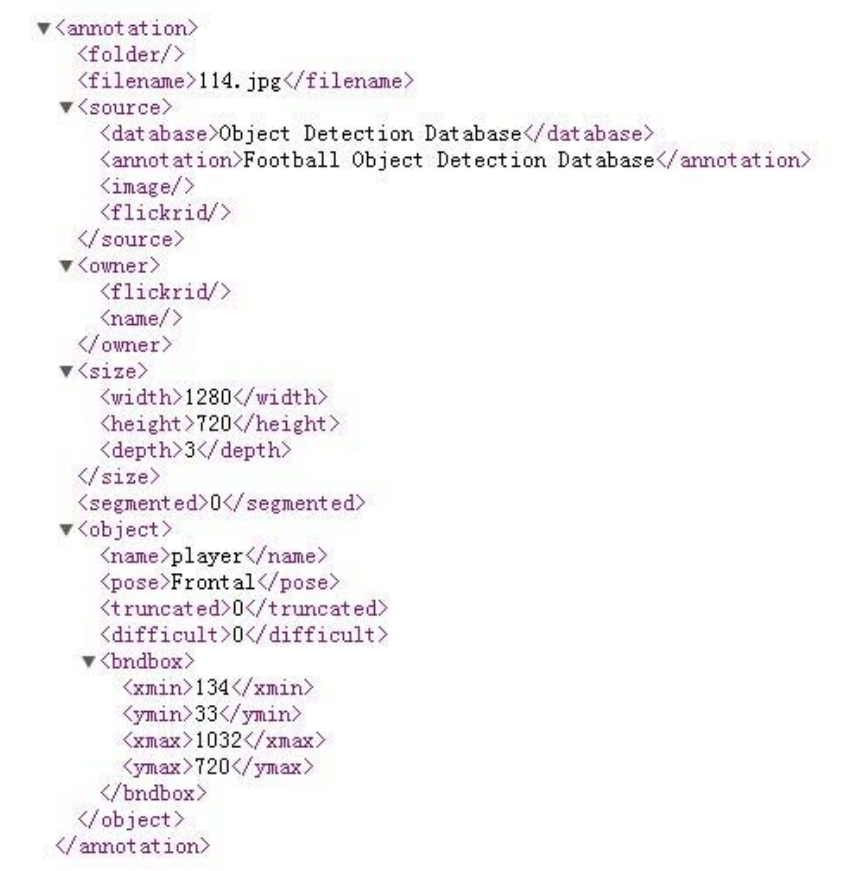
\includegraphics[width=0.8\linewidth]{figuras/MachineLearning/labelXml.png}
	\caption{Arquivo XML gerado pelo LabelImg}
	\legend{Fonte: \citeauthor{zhou2017application} (\citeyear{zhou2017application})}
	\label{fig:labelXml}
\end{figure}

O ImageNet dataset \cite{deng2009imagenet} possui mais de 14 milhões de imagens, cobrindo mais de 20.000 categorias. Existem mais de um milhão de imagens com anotações explícitas de classe e anotações de locais de objetos na imagem. O conjunto de dados Imagenet é um dos conjuntos de dados mais usados no campo da aprendizagem profunda. A maior parte do trabalho de pesquisa, como classificação, localização e detecção de imagens, é baseada nesse conjunto de dados. O conjunto de dados Imagenet é detalhado e é muito fácil de usar. É amplamente utilizado no campo da pesquisa em visão computacional e se tornou o conjunto de dados 'padrão' do aprendizado profundo atual do domínio da imagem para testar o desempenho do algoritmo. \cite{zhou2017application}

O PASCAL VOC (análise de padrões, modelagem estatística e classes de objetos visuais de aprendizado computacional) \cite{everingham2010pascal} fornece conjuntos de dados de imagem padronizados para reconhecimento de classe de objetos e fornece um conjunto comum de ferramentas para acessar os conjuntos de dados e anotações. O conjunto de dados PASCAL VOC inclui 20 classes e tem um desafio baseado nesse conjunto de dados. O PASCAL VOC Challenge \cite{everingham2010pascal} não está mais disponível após 2012, mas seu conjunto de dados é de boa qualidade e bem marcado e permite a avaliação e comparação de diferentes métodos. E como a quantidade de dados do conjunto de dados PASCAL VOC é pequena, comparada ao conjunto de dados imagenet, muito adequada para os pesquisadores testarem programas de rede. Nosso conjunto de dados também é criado com base no padrão de conjunto de dados PASCAL VOC.\cite{zhou2017application}


\subsection{Arquitetura de microsserviços}

Seguindo a definição de \citeauthor{ms1} (\citeyear{ms1}), a arquitetura de microsserviços trata do desenvolvimento de uma aplicação que baseia na existência de diversos pequenos serviços independentes. Cada um dos serviços deve rodar em seu próprio processo independente. Estes serviços podem comunicar entre si utilizando mecanismos leves de comunicação (geralmente em torno no HTTP). Os serviços devem ser absolutamente independentes.

Um exemplo da arquitetura de microsserviços está na Figura \ref{fig:arquitetura-microsservicos}.

\begin{figure}[htbp]
	\centering
	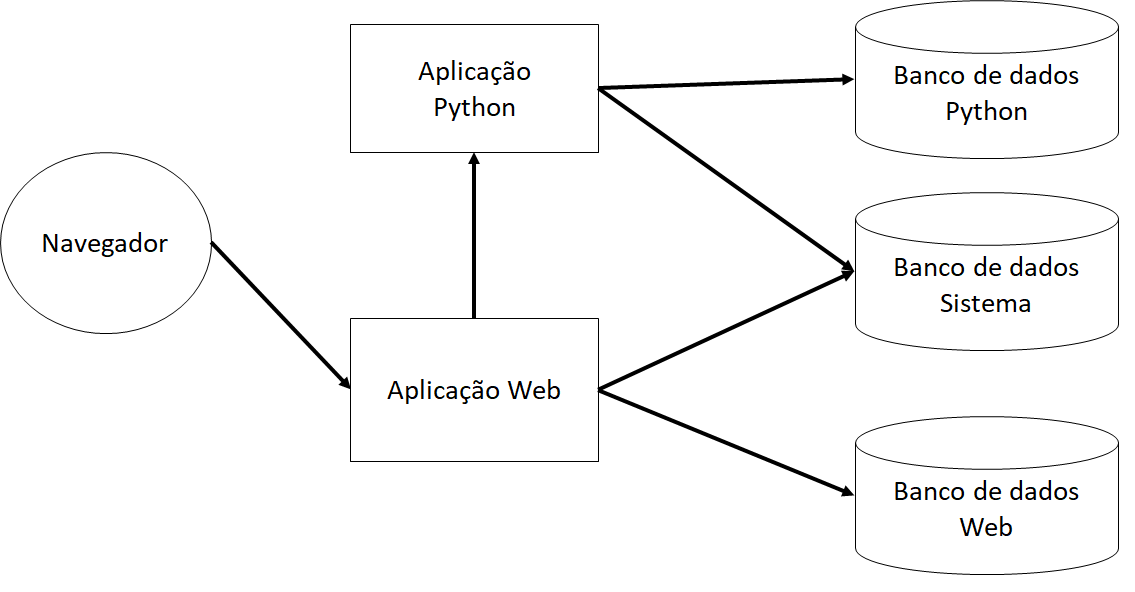
\includegraphics[width=1\linewidth]{figuras/WebService/microservices.png}
	\caption{Exemplo arquitetura de microsserviços.}
	\label{fig:arquitetura-microsservicos}
\end{figure}

Microsserviços são os resultados da decomposição funcional de uma aplicação. São caracterizados pela definição de sua interface e função no sistema. Como cada serviço deve ser independente, uma alteração na sua implementação não deve afetar o funcionamento dos demais. \cite{Pahl}

\subsection{Docker}

Docker é um projeto \textit{open source} que foi inicialmente lançado em 2013, atraiu grande atenção na industria de TI. É uma plataforma de conteinerização que possibilita usuários a construir sua aplicação dentro de um conteiner e transferir conteiners através de máquinas com diferentes sistemas operacionais de um jeito simples. \cite{chang2017kubernetes}

Existem três componentes principais do Docker:

\begin{itemize}
	\item \textit{Docker images}: são \textit{templates} de leitura que servem como base para a criação de conteiners.;
	\item \textit{Docker registries}: é o local onde estão uma grande coleção de \textit{Docker images}.;
	\item \textit{Docker containers}: são as instâncias virtuais em que as aplicações estão rodando. Cada conteiner contem uma aplicação rodando e todas os seus arquivos de dependências, como o código, bibliotecas e utilitários do sistema.
\end{itemize}

A construção de imagens pode ser feita de duas maneiras. É possível criar um conteiner através de uma imagem já existente (\textit{docker run}), realizar modificações e instalações dentro do conteiner, parar o container e depois salvar o estado atual do conteiner como uma nova imagem (\textit{docker commit}). Este processo é parecido com uma instalação clássica de uma máquina virtual, mas deve ser feito para cada imagem caso haja alguma atualização, já que as imagens são padronizadas. Para automatizar o processo, \textit{Dockerfiles} nos permite especificar uma imagem de base e uma sequência de comandos que serão executados quando a imagem é construída, juntamente com outras opções de especificações, como portas a serem expostas. A imagem é depois construída com o comando \textit{docker build}.\cite{DiPietro}
